\documentclass[10pt]{article}

\usepackage[margin=0.9in]{geometry}
\usepackage{amsmath,amssymb}
\usepackage{booktabs}
\usepackage[colorlinks=true,linkcolor=blue,urlcolor=blue]{hyperref}
\usepackage{tikz}
\usetikzlibrary{positioning,arrows.meta,calc}

\newcommand{\eps}{\varepsilon}
\newcommand{\CA}{C_A}
\newcommand{\CF}{C_F}
\newcommand{\as}{\alpha_s}

\title{\vspace{-3ex}Two-loop hard functions for $pp \to h X$:
the workflow in brief}
\author{Max Zhang}
\date{\today}

\begin{document}
\maketitle
\vspace{-4ex}

\paragraph{Goal.}  NNLO (two-loop) partonic hard functions for
single-inclusive hadron production $pp \to h X$ in collinear
factorization at twist two, for unpolarized and polarized channels,
\begin{equation*}
  d\sigma
  = \sum_{a,b,c}
  f_a(x_a) \otimes f_b(x_b) \otimes D_{h/c}(z_h) \otimes
  \hat\omega_{ab\to c}\!\left(x,y;\as,\eps\right),
  \qquad x=-t/s,\;\; y=-u/s,
\end{equation*}
with the twist-two correlators $f_1, g_{1L}, h_1$ (distributions) and
$D_1, G_{1L}, H_1$ (fragmentation), in dimensional regularization with
BMHV $\gamma_5$ (evanescent structures kept exact).  Real radiation is
treated by reverse unitarity: on-shell cuts become cut propagators, so
phase-space integrals reduce like loop integrals, with the endpoint
plus-distribution structure carried in a declared distributional
prefactor.  Currently exercised in full on the NNLO double-real
channel.

\begin{center}
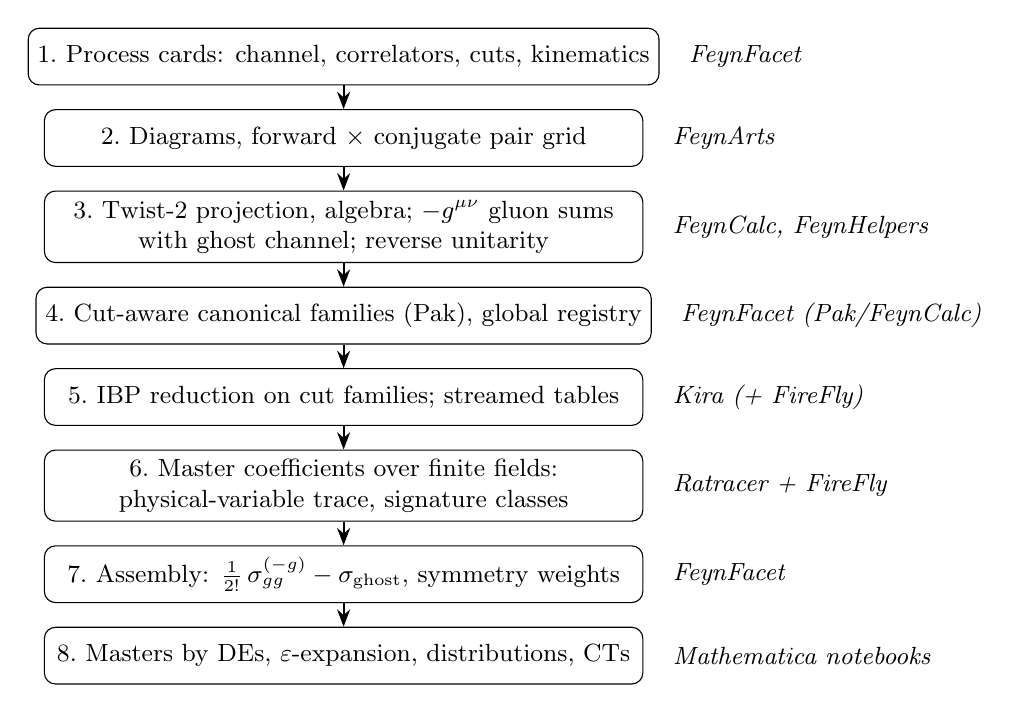
\begin{tikzpicture}[
  stage/.style={draw, rounded corners, align=center,
    minimum width=7.6cm, minimum height=0.72cm, font=\small},
  tool/.style={font=\small\itshape, anchor=west},
  arrow/.style={-{Stealth[length=2.2mm]}, thick},
  node distance=0.30cm
]
\node[stage] (cards) {1.\ Process cards: channel, correlators, cuts,
kinematics};
\node[stage, below=of cards] (diagrams) {2.\ Diagrams, forward
$\times$ conjugate pair grid};
\node[stage, below=of diagrams] (project) {3.\ Twist-2 projection,
algebra; $-g^{\mu\nu}$ gluon sums\\ with ghost channel; reverse
unitarity};
\node[stage, below=of project] (families) {4.\ Cut-aware canonical
families (Pak), global registry};
\node[stage, below=of families] (ibp) {5.\ IBP reduction on cut
families; streamed tables};
\node[stage, below=of ibp] (coeff) {6.\ Master coefficients over
finite fields:\\ physical-variable trace, signature classes};
\node[stage, below=of coeff] (assembly) {7.\ Assembly:
$\tfrac{1}{2!}\,\sigma^{(-g)}_{gg} - \sigma_{\text{ghost}}$, symmetry
weights};
\node[stage, below=of assembly] (masters) {8.\ Masters by DEs,
$\eps$-expansion, distributions, CTs};
\foreach \a/\b in {cards/diagrams, diagrams/project, project/families,
  families/ibp, ibp/coeff, coeff/assembly, assembly/masters}
  \draw[arrow] (\a) -- (\b);
\node[tool] at ($(cards.east)+(0.25,0)$) {FeynFacet};
\node[tool] at ($(diagrams.east)+(0.25,0)$) {FeynArts};
\node[tool] at ($(project.east)+(0.25,0)$) {FeynCalc, FeynHelpers};
\node[tool] at ($(families.east)+(0.25,0)$) {FeynFacet (Pak/FeynCalc)};
\node[tool] at ($(ibp.east)+(0.25,0)$) {Kira (+ FireFly)};
\node[tool] at ($(coeff.east)+(0.25,0)$) {Ratracer + FireFly};
\node[tool] at ($(assembly.east)+(0.25,0)$) {FeynFacet};
\node[tool] at ($(masters.east)+(0.25,0)$) {Mathematica notebooks};
\end{tikzpicture}
\end{center}

\paragraph{Stages.}
\begin{enumerate}\itemsep0.15ex
\item \textbf{Cards} (\textsf{FeynFacet}): declarative definition of a
  channel --- external states, correlators, cut structure, the
  distributional prefactor $f_1 f_1 D_1$ with its endpoint valuations,
  scale, dimensionless $(x,y)$, physical region.  All later stages
  read conventions from the card.
\item \textbf{Diagram pairs} (\textsf{FeynArts}): squared amplitude as
  the full forward $\times$ conjugate grid (NNLO double-real:
  $36\times36$ per channel); pair-level parallelism and resumability.
\item \textbf{Projection} (\textsf{FeynCalc}, \textsf{FeynHelpers}):
  twist-two projectors, Dirac/color reduction to scalar cut
  integrands.  Two-gluon final states use $-g^{\mu\nu}$ polarization
  sums plus a cut ghost--antighost companion channel through the same
  pipeline (Slavnov--Taylor completion; still two loops).
\item \textbf{Canonical families} (\textsf{FeynFacet}, Pak algorithm
  with marked cut propagators): equivalent integral families merged
  into a registry with stable names; gluon and ghost channels share
  one namespace.  NNLO: $1898$ sectors $\to 430$ families.
\item \textbf{IBP} (\textsf{Kira} + \textsf{FireFly}): reduction with
  declared cuts; solved tables streamed and closed family-by-family
  (peak memory set by one family, not the system).  NNLO: $44\,877$
  targets $\to 347$ masters.
\item \textbf{Coefficients} (\textsf{Ratracer} + \textsf{FireFly}):
  exact rational reconstruction of each master's coefficient from
  finite-field probes; see methods below.
\item \textbf{Assembly} (\textsf{FeynFacet}): master-by-master
  combination of channels with identical-particle factors and the
  ghost subtraction; fail-closed on any namespace/measure mismatch.
\item \textbf{Downstream} (notebooks): master integrals by
  differential equations in $(x,y)$, $\eps$-expansion,
  plus-distribution extraction, mass-factorization counterterms
  $\to$ renormalized hard functions.
\end{enumerate}

\paragraph{Coefficient methods (stage 6).}  Contributions carry
half-integer powers of monomials in $(x_a,x_b,s,\dots)$; a square-root
substitution ($x_a=\xi_a^2$, $s=2q^2$, \dots) is applied
\emph{per entry and transiently}: lift, divide the prefactor, cancel,
then descend back via even/odd parts ($N/D = N_e/D_e$ exactly when
$N_eD_o - N_oD_e = 0$), so the reconstruction runs over the physical
variables $\{\CA,\CF,\eps,x,y\}$ only --- root variables would double
the probe degrees.  Scale and $\as$ powers are read off by exact mass
dimension.  Each entry splits as (non-rational
signature)\,$\times$\,(rational function), with signatures identified
\emph{modulo} $\mathbb{Q}(\CA,\CF,\eps,x,y)^\times$
(e.g.\ $b^{m+n\eps} = b^m \cdot (b^\eps)^n$ with $b^m$ folded into the
rational part, canonical per prime): this quotient collapses the
reconstruction to one class per master and scale power.  Probe
\emph{count} is intrinsic (true degrees of the coefficient); probe
\emph{time} is representational (linear in input size), so entries are
exactly canceled in parallel before tracing.

\paragraph{Validation.}  Exact golden regressions at the cheapest
sufficient scale: NLO unpolarized, NLO transversity (evanescent/BMHV
content), and the NNLO ghost channel must be reproduced exactly after
every change.  Sign-definiteness of the rationalization is proved by a
max-flow/min-cut bound (checked numerically).  On a benchmark NNLO
master, the reconstruction matches an independent earlier
implementation in probe count (169.7k vs.\ 169.6k) and wall time.
Status: double-real pipeline complete and validated through the
coefficient stage; ghost channel fully reconstructed; gluon-grid
reconstruction and assembly are the next production steps, followed by
the real-virtual and double-virtual channels through the same stages.

\end{document}
